%%This is a very basic article template.
%%There is just one section and two subsections.
\documentclass[UTF8]{ctexart}
\title{第五章 JESD204B接收端传输层}
\author{陈登}
\date{\today}

\bibliographystyle{plain}
\usepackage{graphicx}
\usepackage{float}
\usepackage{amsmath}
\usepackage{geometry}
\usepackage{fontspec}
\usepackage{algorithm}
\usepackage{algorithmicx}
\usepackage{algpseudocode}

\geometry{a4paper,centering,scale=0.9}
\usepackage[format=hang,font=small,textfont=it]{caption}
\usepackage[toc,page,title,titletoc,header]{appendix}
\usepackage[nottoc]{tocbibind}

\begin{document}

\section{JESD204B接收端传输层设计}

传输层的主要是作为一个承上启下的层面,将下层经过解码、解扰、对齐等操作的序列恢复成发端赋予的具体的转换器数据。
在数据链路层完成了对信道信息的提取后,剩余的就是具体的样本数据,主要包含的是通道位置、样本数等信息。

而对具体数据包的拆包主要是依据各个lane的配置信息,配置信息包含了:
\begin{itemize}
  \item 单个link单个帧时钟周期包含的控制字节数,用CF表示。
  \item 单个转换器样本包含的控制比特数,用CS表示。
  \item 单个lane所包含的转换器数,用L表示。
  \item 单个设备包含的转换器数量,用M表示。
  \item 转换器的分辨率,用N表示。
  \item 单个帧周期单个转换器传输的样本数,用S表示。
\end{itemize}

传输层的具体工作就是根据协议的约定,通过已知的配置信息,将数据链路层得到的数据解包对应到正确的转换器和控制器上。

\subsection{单lane的数据格式}

\subsubsection{没有过采样的情况}

假定一个设备包含M个转换器,每一个样本有N位数据。
MSB位于左端,LSB位于右端。

\begin{enumerate}
	\item 样本采用线性排列,由转换器0开始。
	\item 样本被映射到字,如果需要安排控制字,就存在两种选择,并由CF变量控制:
	\begin{itemize}
		\item 当CF=0时,控制位将会直接加在每个样本的LSB位后。
		\item 当CF=1时,控制位将会组成一个独立的控制字,然后添加在所有样本字之后。控制的第几位就标示第几个转换器的控制位。
	\end{itemize}
	\item 那些不能构成4位整数倍的字被扩展成nibble,在扩展位填充尾比特。这些被扩展的后的字被称作NG,NG的位数必须是4的倍数。
	\begin{itemize}
		\item 当CF=0时,控制位被视作样本字的一部分,所以数据位和控制位之间不存在尾比特位。
		\item 当CF=1时,数据位和控制位在不同的字之中,所以至少有一个尾比特位在每一个样本的数据位后。
	\end{itemize}
	\item 在一些情况下,需要用尾比特位来填充,使得总的位数变成8的倍数。
	\item 最后这些位再重组成F个octet。
\end{enumerate}

以上成帧方式,描述了一个lane里面包含了多个转换器的情况。
相比于之前版本,新的协议在每个样本结尾插入控制位后,在产生octet之前,需要通过nibble扩展重新组成NG,这样导致了更多的octet产生。
所以在接收端处理收到的octects准备还原成数据时需要留意尾部的信息。

具体的组帧理解如图\ref{fig:user_data_format_for_lane_non_oversample}所示。

\begin{figure}[H]
	\centering
	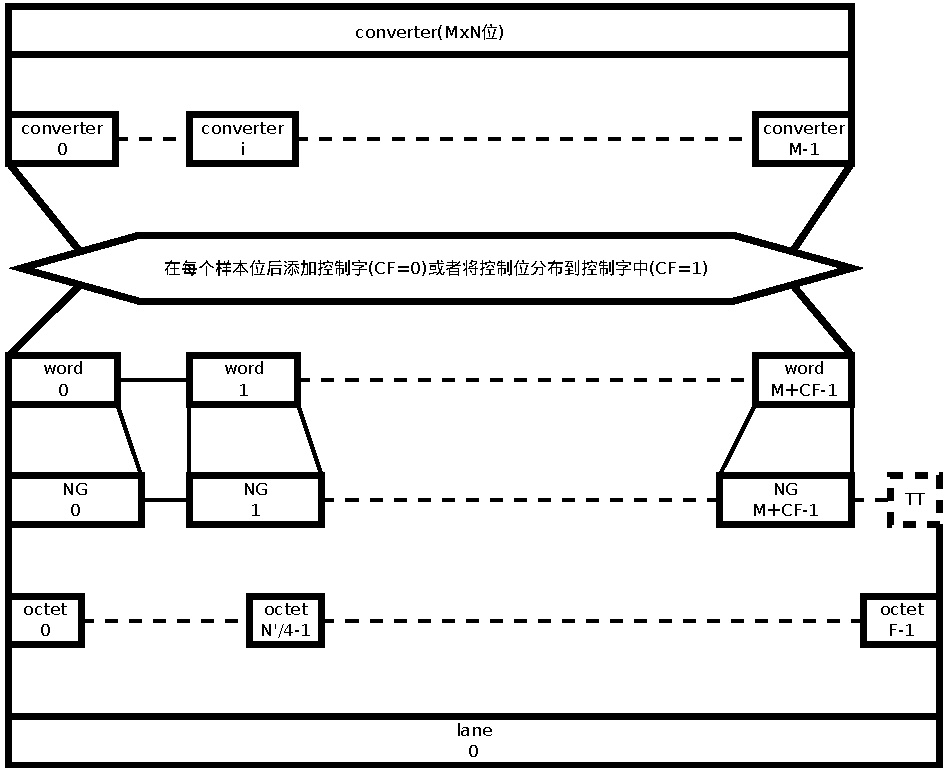
\includegraphics[width=16cm]{./img/user_data_format_for_lane_non_oversample.pdf}
	\caption{单lane没有过采样的组帧方式}
	\label{fig:user_data_format_for_lane_non_oversample}
\end{figure}

可见单个lane当中将多个转换器的转换结果按顺序依次排放,添加完尾比特和控制位后完整的传输。
一个转换器同一时刻只对应一个样本,不存在过采样的情况。

具体的组帧格式如图\ref{fig:user_data_format_with_control_word}所示。

\begin{figure}[H]
	\centering
	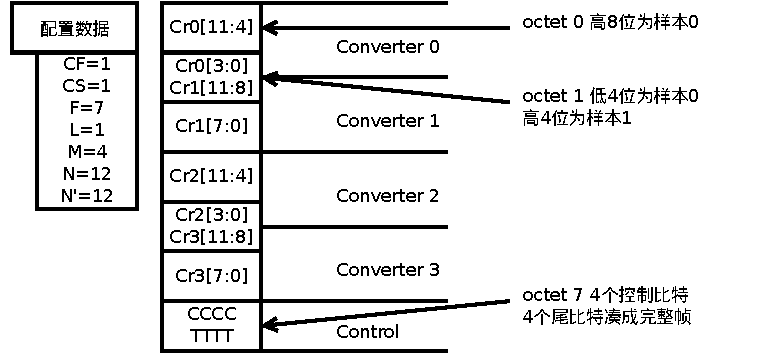
\includegraphics[width=16cm]{./img/user_data_format_with_control_word.pdf}
	\caption{有控制字的用户数格式}
	\label{fig:user_data_format_with_control_word}
\end{figure}

根据CS=1可以知道,每个转换样本要包含1个控制位,这一控制位直接添加在转换结果后。
根据CF=1可以知道,每个link的每个帧中只包含1个控制字,这一控制字根据CS=1分布在各个样本中。

\subsubsection{有过采样的情况}

映射的方法类似于没有过采样的lane。
实际上有过采样的lane相当于每一个转换器一次采集了S个样本。
这样造成的区别就是样本的排列顺序,第一个转换器采集了S个样本,那么这S个样本就先按顺序排列直接去组成字,然后再处理下一个转换器的样本。
之后的nibble扩展和octet拆分都与没有过采样的相同。

\subsection{多lane的数据格式}

假如一个link有多个lane,就存在多lanes的成帧问题。
对于含有L个lane的link,对于单个lane的映射方式是相同的。
不同在于最后形成一串L×F个octet的数据。
最先的F个octet在lane 0上传输,接下来的F个octet在lane 1上传输,以此类推。

相较于独立lane的格式,多lanes需要添加一些特殊的信息。
\begin{enumerate}
	\item 参数HD决定了一个样本是否分配到不同的lane中。
	\begin{itemize}
		\item 在低密度模式下\footnote{Low Density mode, HD=0},位于F octects尾部的字不需要补充tail位在最后一个完整NG之后。
		\item 在高密度模式下\footnote{High Density mode, HD=1}转换完成的字可能会被拆分,有可能进入不同的lane。
	\end{itemize}
	\item 参数CF决定了每一个帧周期内每个连接的控制字数量,在多lane模式下,它也决定了哪一个lane用来传输控制字。
	\begin{itemize}
		\item 当CF=0时,表示不存在控制字,控制信息分散在每一个数据字中。
		\item 当CF!=1时,CF作为L和M的分母。将所有的lanes分成L组,每一组包含L/CF个lanes,在每一个CF组里面有M/CF个转换器。在这M/CF个转换器产生的SxM/CF个样本后插入一个控制字,这个控制字d即包含了之前连续SxM/CF个样本的控制信息。如果控制字刚好与单个lane吻合,则不允许被lane拆分。
	\end{itemize}
\end{enumerate}

没有控制字情况下,具体的组帧格式如图\ref{fig:multilane_user_data_format_without_control_word}所示。

\begin{figure}[H]
	\centering
	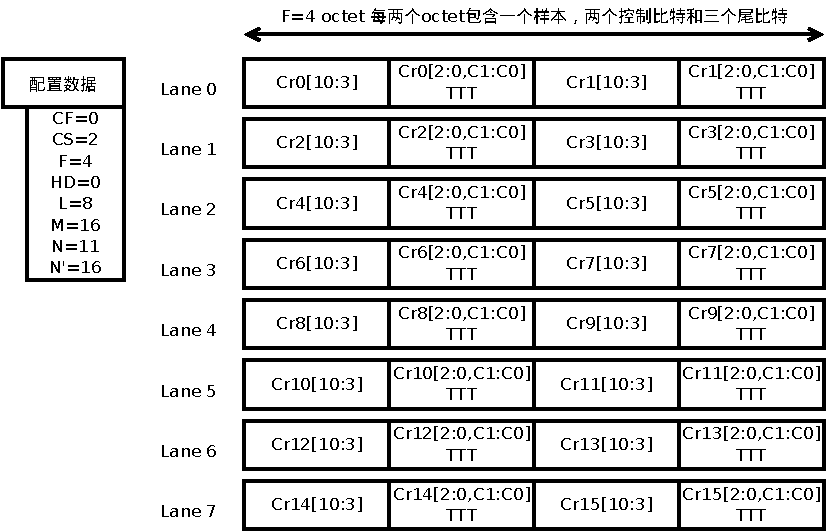
\includegraphics[width=16cm]{./img/multilane_user_data_format_without_control_word.pdf}
	\caption{多lane没有控制字的用户数格式}
	\label{fig:multilane_user_data_format_without_control_word}
\end{figure}

有控制字情况下,具体的组帧格式如图\ref{fig:multilane_user_data_format_with_two_control_words}所示。

\begin{figure}[H]
	\centering
	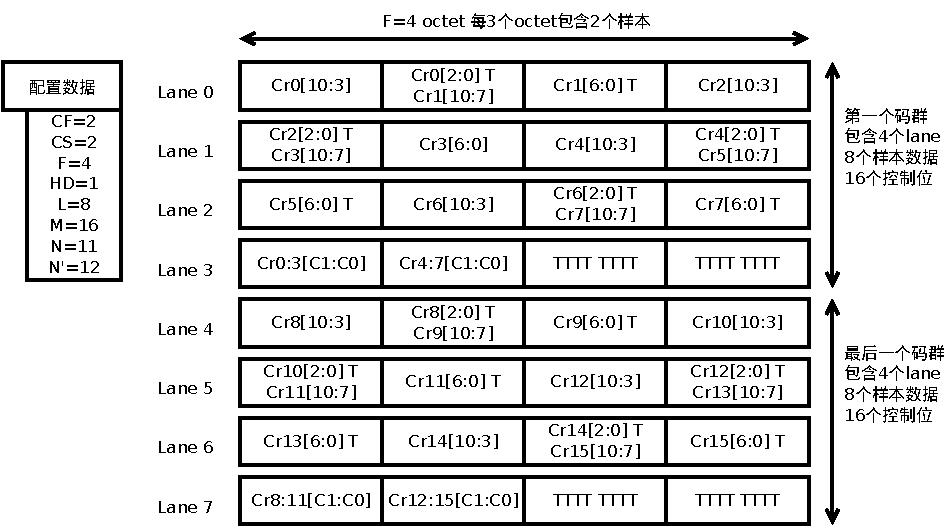
\includegraphics[width=16cm]{./img/multilane_user_data_format_with_two_control_words.pdf}
	\caption{多lane有控制字的用户数格式}
	\label{fig:multilane_user_data_format_with_two_control_words}
\end{figure}

\subsection{尾比特}

尾比特位是在加扰前添加的,当需要加扰时他同数据位一起加扰。
为了避免这些尾比特位对帧同步符号性能的影响,它们必须满足以下要求:

\begin{itemize}
	\item 每个帧的尾比特位都是相同的,或者
	\item 都是由至少9阶多项式的伪随机序列生成器生成
\end{itemize}

所以说,如果不加扰的话,尾比特位可能会导致线性频谱。

\subsection{空闲模式}

空闲模式就是有一个以上的转换器连接到同一个link上,不过它们有的是未被激活的或者说启用的。
不过它们的接口是存在的,并且帧的结构并没有改变。

对于每个link拥有多个转换器的系统,可能出现一个转换器和别的转换器共享它的octet。
这样说来的话,如果一个转换器没被启用,那么他将不能通过8B/10B编码的控制字符,被标志在数据链路层上。
也就是说,接收方无法知道这个转换器是否被启用。
这就需要一个特殊的控制位来说明这一点,但也可以通过控制位来传递这一信息。

未被激活的转换器所传输的数据被称作Dummy样本。
对于Dummy样本的唯一要求就是不能阻止生成对齐符号。
Dummy样本可能由应用层生成,但这样就无法确认它是否会被映射到帧的最后一个octet,从而产生不应该存在的对齐符号。
为了避免这一情况,Dummy样本应该满足和尾比特位一样的要求。
伪随机序列是一个很好的选择,这样可以避免在加扰被关闭的情况下产生的频谱峰值。
另一个选择就是传输传输层测试序列。

\bibliography{../../bib/serdes}
\end{document}
